% Use only LaTeX2e, calling the article.cls class and 12-point type.

\documentclass[12pt]{article}

% Users of the {thebibliography} environment or BibTeX should use the
% scicite.sty package, downloadable from *Science* at
% www.sciencemag.org/about/authors/prep/TeX_help/ .
% This package should properly format in-text
% reference calls and reference-list numbers.

\usepackage{scicite}

% Use times if you have the font installed; otherwise, comment out the
% following line.

\usepackage{times}

% The preamble here sets up a lot of new/revised commands and
% environments.  It's annoying, but please do *not* try to strip these
% out into a separate .sty file (which could lead to the loss of some
% information when we convert the file to other formats).  Instead, keep
% them in the preamble of your main LaTeX source file.

\usepackage{graphicx}

% The following parameters seem to provide a reasonable page setup.

\topmargin 0.0cm
\oddsidemargin 0.2cm
\textwidth 16cm 
\textheight 21cm
\footskip 1.0cm


%The next command sets up an environment for the abstract to your paper.

\newenvironment{sciabstract}{%
\begin{quote} \bf}
{\end{quote}}


% If your reference list includes text notes as well as references,
% include the following line; otherwise, comment it out.

\renewcommand\refname{References and Notes}

% The following lines set up an environment for the last note in the
% reference list, which commonly includes acknowledgments of funding,
% help, etc.  It's intended for users of BibTeX or the {thebibliography}
% environment.  Users who are hand-coding their references at the end
% using a list environment such as {enumerate} can simply add another
% item at the end, and it will be numbered automatically.

\newcounter{lastnote}
\newenvironment{scilastnote}{%
\setcounter{lastnote}{\value{enumiv}}%
\addtocounter{lastnote}{+1}%
\begin{list}%
{\arabic{lastnote}.}
{\setlength{\leftmargin}{.22in}}
{\setlength{\labelsep}{.5em}}}
{\end{list}}


% Include your paper's title here

\title{Interim Report} 


% Place the author information here.  Please hand-code the contact
% information and notecalls; do *not* use \footnote commands.  Let the
% author contact information appear immediately below the author names
% as shown.  We would also prefer that you don't change the type-size
% settings shown here.

\author
{Radek Chramosil\\
\\
\normalsize{WorldQuant University}\\
\\
\normalsize{E-mail:  radek@keemail.me}
}

% Include the date command, but leave its argument blank.

\date{}



%%%%%%%%%%%%%%%%% END OF PREAMBLE %%%%%%%%%%%%%%%%



\begin{document} 

% Double-space the manuscript.

\baselineskip24pt

% Make the title.

\maketitle 



% Place your abstract within the special {sciabstract} environment.

\begin{sciabstract}
This document is the Interim Report for the Capstone Project. It shows the basic structure for the database that holds data the data from crypto-currency exchange Binance and some initial data analysis.
\end{sciabstract}

% In setting up this template for *Science* papers, we've used both
% the \section* command and the \paragraph* command for topical
% divisions.  Which you use will of course depend on the type of paper
% you're writing.  Review Articles tend to have displayed headings, for
% which \section* is more appropriate; Research Articles, when they have
% formal topical divisions at all, tend to signal them with bold text
% that runs into the paragraph, for which \paragraph* is the right
% choice.  Either way, use the asterisk (*) modifier, as shown, to
% suppress numbering.

\section*{Introduction}
The structure of the database is described below. Additionally,  I provide more details about the data analyses so far carried out as well as some suggestion for trading possible trading strategies. Some plots for second data set are provided. The asset I worked with is \textbf{TUSDBTC} as quoted on \textit{Binance Exchange}. The asset is Bitcoin quoted in USD. The access to the full exchange is free and level 2 data is available for every tick. The data was collected on second basis for one hour. The collection was done with 1 second frequency as opposed to per trade basis (I am still unsure how to handle data collection per trade basis). The data set is therefore some 3440 full market book hits; some 100 quotes for bid prices and some 100 quotes for ask prices.

\pagebreak

\section*{Database Structure}
I have included the below tables in this submission. The tables can be created by SQL commands in the ``create\_db.sql`` file. The schema for the database is shows in Figure \ref{fig:schema}.\\
\begin{figure}[h!]
  \centering
  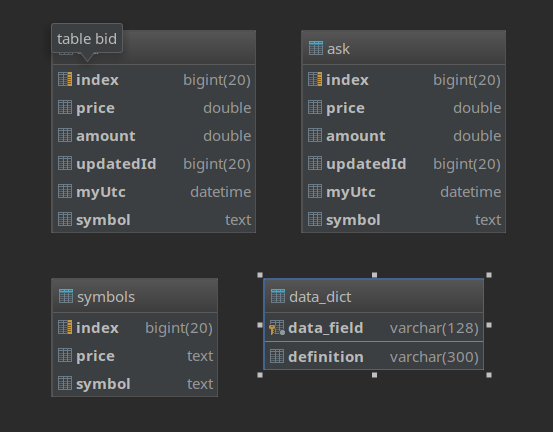
\includegraphics[scale=0.40]{schema.png}
  \caption{Schema}
  \label{fig:schema}
\end{figure}

The tables can be dropped using the ``rollback\_db.sql`` file. This file provides a logical inverse to the create operation. Additionally, I built functionality that can create table on fly using Pandas and SQL Alchemy however the default behaviours are not very good as it fails to create foreign keys and so on.

\subsection*{Tables}
\paragraph*{symbolRef.} This is just a reference table for symbols. The symbols are strings, however it is more efficient to use integers for foreign keys and it is better to store integers than strings.
\paragraph*{bid and ask.} These to table are identical from data types point of view however the just store the bid and ask prices as well as my UTC time stamp and the server `updatedId` flag. This is a large integer that gets changed each time there is a trade.
\paragraph*{limits.}. Basically, the exchange give users request or order limits in time intervals. We can make 1200 data request in a minute or 10 orders in a second and 100 000 orders in a day. If we are creating a real trading application we would have to consider these closely.
\paragraph*{data\_dict.} This is manually created table and holds descriptions for the data fields in the database.

\section*{Bid and Ask}
Bid and ask prices are split into two tables. The tables are identical. The tables from Figure \ref{fig:ask} and Figure \ref{fig:bid} carry the data for the symbol and specific Exchange ID as given by \textit{updateId} column. My time stamps are in the \textit{myUtc} column representing the time on my computer.

\begin{figure}[h!]
	\centering
  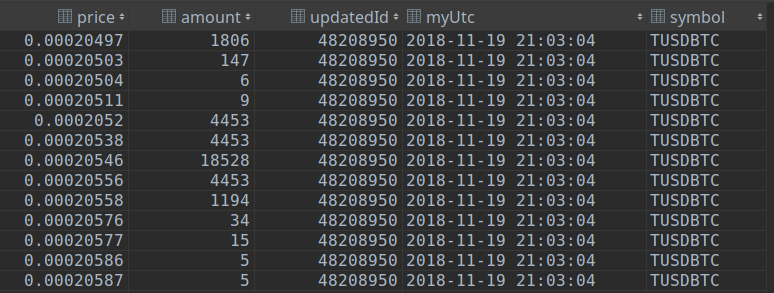
\includegraphics[scale=0.3]{ask.png}
  \caption{Ask Price}
  \label{fig:ask}
\end{figure}

\begin{figure}[h!]
	\centering
  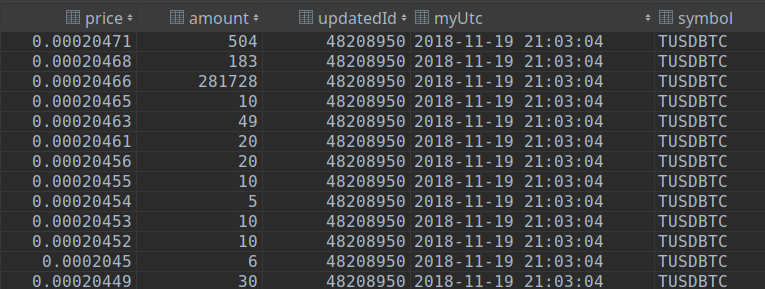
\includegraphics[scale=0.3]{bid.png}
  \caption{Bid Price}
  \label{fig:bid}
\end{figure}

\section*{Exchange API}
It is important to handle the communication to the Exchange well. The class \textit{DataEndPoint} hold all methods that can collect the data from the exchange as opposed to submit trades. I leave it to the reader to read over the comments for these methods to see what can be easily pulled out from the exchange.

\section*{Data Analysis - First Look}
I collected 1 hour of trading data on per second basis. Figure \ref{fig:plt1} shows cumulative bid and ask prices with quantity. The way how I think about this is it is supply and demand curves. We see that there is a lot of volatility over 1 minute interval. This is good as it means that we will be able to create strategies.
\begin{figure}[h!]
	\centering
  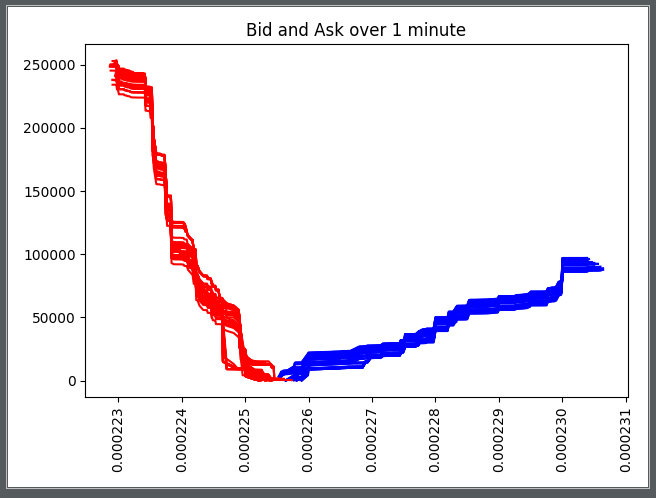
\includegraphics[scale=0.5]{plot1.png}
  \caption{All bid and ask prices and quantities in 1 minute}
  \label{fig:plt1}
\end{figure}

The problem in the Figure \ref{fig:plt1} is that we do not see much details. So, I plotted the same time interval but with close look at what was happing around the spread in Figure \ref{fig:plt2}. Again we see the volatility in the price within one minute.

\begin{figure}[h!]
	\centering
  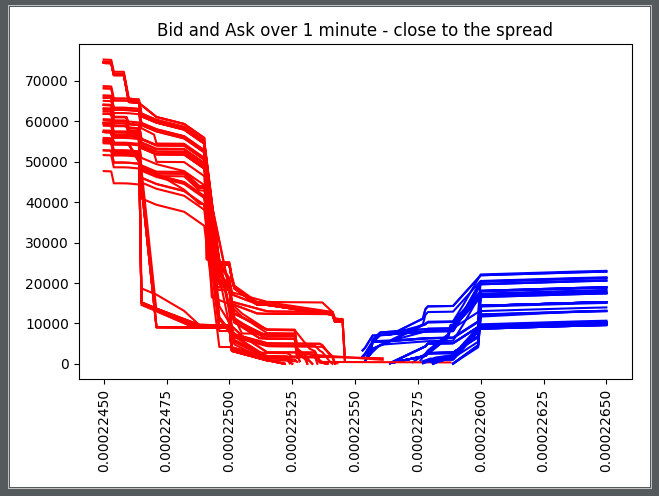
\includegraphics[scale=0.5]{plot2.png}
  \caption{Detailed Price and quantity moments around the spread in 1 minute}
  \label{fig:plt2}
\end{figure}

We also have have look the maximum bid and minimum ask prices and plot them over the 1 hour interval. This is plotted in Figure \ref{fig:plt3}. This shows that we do have trends and turning points happing over time again. We should use the trading strategies that we learning for this and we can starting simulating the trade at bid and ask prices.

\begin{figure}[h!]
	\centering
  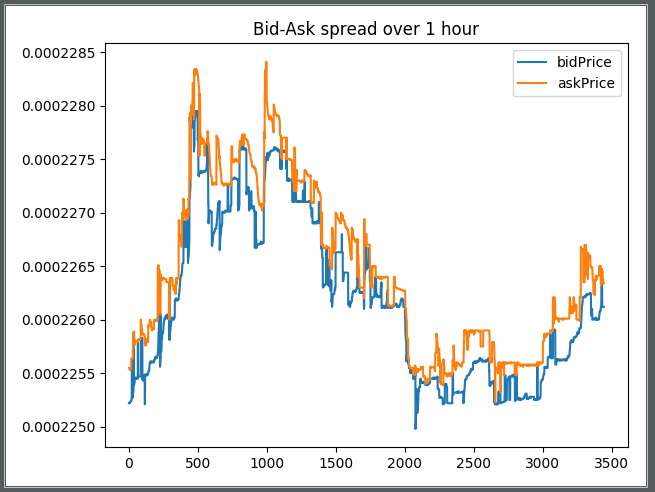
\includegraphics[scale=0.5]{plot3.png}
  \caption{Max bid and min ask over 1 hour}
  \label{fig:plt3}
\end{figure}

Finally, we check the spread for the two currencies as in Figure \ref{fig:plt4}. We immediately see that that we could create mean reversion strategy for the spread. It may not be viable on profit versus fee basis however we could tests this.

\begin{figure}[h!]
	\centering
  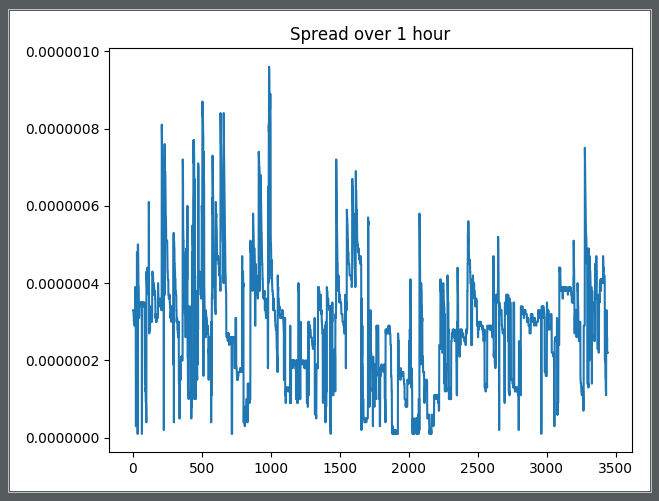
\includegraphics[scale=0.5]{plot4.png}
  \caption{Max bid and min ask spread over 1 hour}
  \label{fig:plt4}
\end{figure}

\section*{Some Research - to be done}
Please advise how important this is. I focus on coding over last two weeks.
\subsection{Electronic Trading Chain}
\label{sec:Chian}
\subsubsection{Exchanges}
\subsubsection{Brokers}
\subsubsection{Algo. Trading engines}
\subsubsection{DMA Services}
\subsection{Benefits and Pitfalls of DMA technologies}
\subsubsection{Automated Order Routing systems - AORs}
\subsubsection{Sponsored Access - SA}
\subsubsection{Direct access by non-intermediary market-members}
\subsection{Risks in DMA}
\subsection{Latency Types}
\subsubsection{Transmission Latency}
\subsubsection{Propagation Latency}
\subsubsection{Processing Latency}
\subsection{Typical Order Messaging System}
\label{sec:Messaging}

\pagebreak
\section*{Summary}
Looking at the data, it is easy to spot the same patters as in the time frequencies however connecting to the exchange directly gives full details as to what is going in the market. We are not able to do this for equity or standard financial markets for free. Having a look at the data, we will be able to exactly model what is going in the market rather than second guess from some summary data such as OHLC from Yahoo.
Going forwards, I will focus on creating and testing at least one trading strategy in the data.

\end{document}




















